% -*- coding: utf-8 -*-

\part{Specifications Database}

\chapter{Overview}

\paragraph{%
In knowing how to maintain any system, it is critical to know what the expected %
behaviour of that system is. Hence, this section of the book contains data on the %
stock configuration of all Old World Macintosh models (Performa-branded %
Macintoshes are not covered due to their being variations on a base model, %
a full listing will be present.) % 
}

\paragraph{%
This database is chiefly divided into two segments, for ease of navigation. The %
first, ``68k Macintoshes'', covers Macintoshes making use of the Motorola 68000 %
series microprocessors. These are identified by a lack of \textsl{\textbf{\textrm{PowerPC}}} %
branding on the case of the machine. The second segment, ``PowerPC Macintoshes'', %
covers Power Macintoshes and PowerBooks bearing the \textsl{\textbf{\textrm{PowerPC}}} logo; % 
these machines make use of a high-performance RISC CPU series principally designed by IBM. %
}

\paragraph{%
The data in the following pages is definitive, verified against multiple sources, including %
(where possible) the author's own collection. For machines not in the author's collection, %
data is provided based on at least two sources, three if possible, in order to minimise the %
risk of false information. The only disputable data is what constitutes the ``Optimal'' %
System Software version for a given Macintosh; this is based on the author's own %
experience and is entirely arbitrary. Caveat lector, your mileage may vary. %
}

\cleardoublepage
% -*- coding: utf-8 -*-

\chapter{68k Macintoshes}

\begin{center}
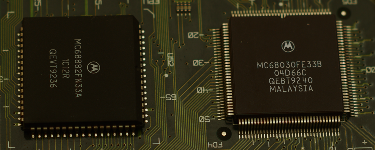
\includegraphics[height=1in]{68k/68030-68882-33.pdf} \\
\end{center}

\paragraph{\scriptsize{\textsc{%
68030 CPU and 68882 FPU from a Macintosh IIvx. This combination %
was used in many 68k Macintoshes to great effect. An FPU such as %
the one depicted here can improve performance in some applications %
by up to 80 percent.}}}

\paragraph{%
The Motorola 68000 series microprocessors were at the heart of every Macintosh %
until early 1994, when the first PowerPC-based workstations, known as Power %
Macintoshes, were released. Even after the release of the wildly successful %
Power Macintosh line, Macintoshes built around the 68040 were sold until %
their discontinuation in October of 1996. %
}

\paragraph{%
The Motorola 68000 microprocessor was, a full decade after its introduction to %
market, regarded widely as one of the most powerful and versatile production %
microprocessors available. It is worth noting that in this decade the %
significantly enhanced 68020 and 68030 had started to enjoy widespread use %
in workstations; no small praise then that the 68000 should stay relevant! %
}

\paragraph{%
On the topic of workstations, it is important to note a special machine which %
will not be covered in this text; the Macintosh XL. Ostensibly a repurposed %
Apple Lisa 2/10 with an Emulation Package allowing for the seamless execution %
of well-behaved Macintosh Software, the XL is not a Macintosh in the truest %
sense of the term; rather it is an inelegant attempt to recoup costs on a %
failed product. Aside from that attempting Lisa repairs or service in this %
day and age is an insane (not insanely great, merely insane) proposition, the %
Lisa falls outside the scope of this text. Information on the Lisa is, however, %
plentiful, if you know where to look, and I strongly encourage you to do so, if %
only to get a glimpse of what was a groundbreaking computer in its time. %
}

\paragraph{%
Several 68k microprocessors have been manufactured by Motorola over the years, %
and not all of them enjoy electrical similarities or code-compatibility. As such, %
it is important to note the particular microprocessors you will be dealing with. %
68000-series microprocessors likely to be found in the 68k Macintoshes you will %
come across are the 68000, 68020, 68030, 68LC040, and 68040. % 
}

% Compact Macs
% -*- coding: utf-8 -*-

\chapter{Compact Macs}

% -*- coding: utf-8 -*-

\section{Macintosh}
\sectionrule

\begin{tabular}{ r p{6in} }
\textbf{Gestalt/Machine ID} & \textbf{1} \\
\textbf{Model Numbers:} & M0001 (Macintosh) \\
\\
\textbf{Graphics:} & Macintosh Framebuffer, 512\(\times\)342 1bpp \\
\textbf{Display:} & Internal, 9'' CRT \\
\\
\textbf{System Bus:} & 8 MHz \\
\textbf{Processors:} & Motorola 68000 ( 8 MHz ) \\
\\
\textbf{Cache Memory:} & None \\
\textbf{RAM (Logic Board):} & 128 kB \\
\textbf{RAM Type:} & PDIP-16 150ns DRAM \\
\\
\textbf{Floppy Drive:} & 400kB 3.5'' SS,DD; GCR \\
\textbf{Optical Drive:} & None \\
\textbf{Hard Drive:} & None \\
\textbf{Other Drives:} & None \\
\textbf{External:} & Apple HD20 (via ext. floppy) \\
~ & Macintosh External Disk Drive (M0130) (ext. floppy) \\
\\
\textbf{PRAM Battery:} & Type 523 (4.5V Alkaline) \\
~ & ( Mallory PX21, IEC 3LR50, ANSI 1306A )\\
\textbf{Power Supply:} & 60W, Integrated \\
%\textbf{Nubus Slots:} & 0 \\
%\textbf{PDS Slot:} & LC PDS \\
\\
%\textbf{Comm Slot:} & Comm Slot Type I \\
%\textbf{Modem:} & \\
%\textbf{Ethernet:} & \\
%\\
\textbf{Input:} & Keyboard, RJ-11 connector \\
~ & Mouse, Serial (custom), DE-9 connector \\
\\
\textbf{Serial Ports:} & 2 \(\times\) RS-422, DE-9 connector \\
\textbf{External Storage:} & IWM interface, DA-19 connector \\
\textbf{Audio:} & 1 \(\times\) Mono output, 3.5mm TS connector \\
\\
\textbf{\textsc{System Software}} & ~ \\
\textbf{Firmware:} & Macintosh ROM (64k) \\
\textbf{Original:} & System 1.0 | Finder 1.0 \\
%\textbf{Optimal:} & ~ \\
\textbf{Latest Supported:} & System 3.2 | Finder 5.3 \\
%\textbf{Latest Possible:} & ~ \\
\end{tabular}
% -*- coding: utf-8 -*-

\section{Macintosh 512k}
\sectionrule

\begin{tabular}{ r p{6in} }
\textbf{Gestalt/Machine ID} & \textbf{2} (512k) \\
~ & \textbf{3} (512ke) \\
\textbf{Model Numbers:} & M0001W (Macintosh 512k) \\
~ & M0001E (Macintosh 512ke) \\
~ & M0001D (Macintosh 512k/800) \\
~ & M0001ED (Macintosh 512ke EDU) \\
\\
\textbf{Graphics:} & Macintosh Framebuffer, 512\(\times\)342 1bpp \\
\textbf{Display:} & Internal, 9'' CRT \\
\\
\textbf{System Bus:} & 8 MHz \\
\textbf{Processors:} & Motorola 68000 ( 8 MHz ) \\
\\
\textbf{Cache Memory:} & None \\
\textbf{RAM (Logic Board):} & 128 kB \\
\textbf{RAM Type:} & PDIP-16 150ns DRAM \\
\\
\textbf{Floppy Drive:} & \textbf{[512k]} 400kB 3.5'' SS,DD; GCR \\
~ & \textbf{[512ke]} 800kB 3.5'' DS,DD; GCR \\
\textbf{Optical Drive:} & None \\
\textbf{Hard Drive:} & None \\
\textbf{Other Drives:} & None \\
\textbf{External:} & Apple HD20 (via ext. floppy) \\
~ & Macintosh External Disk Drive (M0131) (ext. floppy) \\
\\
\textbf{PRAM Battery:} & Type 523 (4.5V Alkaline) \\
~ & ( Mallory PX21, IEC 3LR50, ANSI 1306A )\\
\textbf{Power Supply:} & 60W, Integrated \\
%\textbf{Nubus Slots:} & 0 \\
%\textbf{PDS Slot:} & LC PDS \\
\\
%\textbf{Comm Slot:} & Comm Slot Type I \\
%\textbf{Modem:} & \\
%\textbf{Ethernet:} & \\
%\\
\textbf{Input:} & Keyboard, RJ-11 connector \\
~ & Mouse, Serial (custom), DE-9 connector \\
\\
\textbf{Serial Ports:} & 2 \(\times\) RS-422, DE-9 connector \\
\textbf{External Storage:} & IWM interface, DA-19 connector \\
\textbf{Audio:} & 1 \(\times\) Mono output, 3.5mm TS connector \\
\\
\textbf{\textsc{System Software}} & ~ \\
\textbf{Firmware:} & Macintosh ROM (64k) \\
\textbf{Original:} & \textbf{[512k]} System 1.1 | Finder 1.1g \\
~ & \textbf{[512ke]} System 3.0 | Finder 5.1 \\
%\textbf{Optimal:} & ~ \\
\textbf{Latest Supported:} & \textbf{[512k]} System 4.1 | Finder 5.5 \\
~ & \textbf{[512ke]} System 6.0.8 \\
%\textbf{Latest Possible:} & ~ \\
\end{tabular}
% -*- coding: utf-8 -*-

\section{Macintosh Plus}
\sectionrule

\begin{tabular}{ r p{6in} }
\textbf{Gestalt/Machine ID} & \textbf{4} \\
\textbf{Model Numbers:} & M0001A (Macintosh Plus) \\
\\
\textbf{Graphics:} & Macintosh Framebuffer, 512\(\times\)342 1bpp \\
\textbf{Display:} & Internal, 9'' CRT \\
\\
\textbf{System Bus:} & 8 MHz \\
\textbf{Processors:} & Motorola 68000 ( 8 MHz ) \\
\\
\textbf{Cache Memory:} & None \\
\textbf{RAM (Logic Board):} & None \\
\textbf{RAM Ceiling:} & 4MB \\
\textbf{RAM Type:} & 150ns DRAM - 4 \(\times\) 30-pin SIMM \\
\\
\textbf{Floppy Drive:} & 800kB 3.5'' DS,DD; GCR \\
\textbf{Optical Drive:} & None \\
\textbf{Hard Drive:} & None \\
\textbf{Other Drives:} & None \\
\textbf{External:} & Apple HD20 (via ext. floppy) \\
~ & Macintosh External Disk Drive (M0131) (ext. floppy) \\
\\
\textbf{PRAM Battery:} & Type 523 (4.5V Alkaline) \\
~ & ( Mallory PX21, IEC 3LR50, ANSI 1306A )\\
\textbf{Power Supply:} & 60W, Integrated
%\textbf{Nubus Slots:} & 0 \\
%\textbf{PDS Slot:} & LC PDS \\
\\
%\textbf{Comm Slot:} & Comm Slot Type I \\
%\textbf{Modem:} & \\
%\textbf{Ethernet:} & \\
%\\
\textbf{Input:} & Keyboard, RJ-11 connector \\
~ & Mouse, Serial (custom), DE-9 connector \\
\\
\textbf{Serial Ports:} & 2 \(\times\) RS-422, DE-9 connector \\
\textbf{External Storage:} & IWM interface, DA-19 connector \\
~ & SCSI-I, DB-25 connector \\
\textbf{Audio:} & 1 \(\times\) Mono output, 3.5mm TS connector \\
\\
\textbf{\textsc{System Software}} & ~ \\
\textbf{Firmware:} & Macintosh ROM (128k) \\
\textbf{Original:} & System 3.0 | Finder 5.1 \\
\textbf{Optimal:} & System 6.0.8 \\
\textbf{Latest Supported:} & System 7.5.5 \\
%\textbf{Latest Possible:} & ~ \\
\end{tabular}
% -*- coding: utf-8 -*-

\section{Macintosh SE}
\sectionrule

\begin{tabular}{ r p{6in} }
\textbf{Gestalt/Machine ID} & \textbf{5} \\
\textbf{Model Numbers:} & M5010 (Macintosh SE) \\
~ & M5011 (Macintosh SE FDHD) \\
\\
\textbf{Graphics:} & Macintosh Framebuffer, 512\(\times\)342 1bpp \\
\textbf{Display:} & Internal, 9'' CRT \\
\\
\textbf{System Bus:} & 8 MHz \\
\textbf{Processors:} & Motorola 68000 ( 8 MHz ) \\
\\
\textbf{Cache Memory:} & None \\
\textbf{RAM (Logic Board):} & None \\
\textbf{RAM Ceiling:} & 4MB \\
\textbf{RAM Type:} & 150ns DRAM - 4 \(\times\) 30-pin SIMM \\
\\
\textbf{Floppy Drive:} & \textbf{[SE]} 2 \(\times\) 800kB 3.5'' DS,DD; GCR \\
~ & \textbf{[SE FDHD]} 1.44MB 3.5'' SuperDrive \\
\textbf{Optical Drive:} & None \\
\textbf{Hard Drive:} & \textbf{[SE]} Optional, replaces second floppy drive \\
~ & \textbf{[SE FDHD]} 20MB or 40MB SCSI \\
\textbf{Other Drives:} & None \\
\textbf{External:} & Apple HD20 (via ext. floppy) \\
~ & Macintosh External Disk Drive (M0131) (ext. floppy) \\
\\
\textbf{PRAM Battery:} & \sfrac{1}{2}AA 3.6V \ce{Li}-\ce{SOCl2} \\
~ & ( SAFT LS14250, IEC ER14250, Tadiran TL5101 ) \\
\textbf{Power Supply:} & 100W \\
\\
%\textbf{Nubus Slots:} & 0 \\
\textbf{PDS Slot:} & SE PDS \\
%\textbf{Comm Slot:} & Comm Slot Type I \\
%\textbf{Modem:} & \\
%\textbf{Ethernet:} & \\
%\\
\textbf{Input:} & Apple Desktop Bus, MiniDIN-4K connector \\
\\
\textbf{Serial Ports:} & 2 \(\times\) RS-422, MiniDIN-8 connector \\
\textbf{External Storage:} & IWM interface, DA-19 connector \\
~ & SCSI-I, DB-25 connector \\
\textbf{Audio:} & 1 \(\times\) Mono output, 3.5mm TS connector \\
\\
\textbf{\textsc{System Software}} & ~ \\
\textbf{Firmware:} & Macintosh ROM (256k) \\
\textbf{Original:} & System 4.0 | Finder 5.4 \\
\textbf{Optimal:} & System 6.0.8 \\
\textbf{Latest Supported:} & System 7.5.5 \\
%\textbf{Latest Possible:} & ~ \\
\end{tabular}
% -*- coding: utf-8 -*-

\section{Macintosh SE/30}
\sectionrule

\begin{tabular}{ r p{6in} }
\textbf{Gestalt/Machine ID} & \textbf{9} \\
\textbf{Model Numbers:} & M5119 (Macintosh SE/30) \\
\\
\textbf{Graphics:} & Macintosh Framebuffer, 512\(\times\)342 1bpp \\
\textbf{Display:} & Internal, 9'' CRT \\
\\
\textbf{System Bus:} & 16 MHz \\
\textbf{Processors:} & Motorola 68030 ( 16 MHz ) \\
~ & Motorola 68882 ( 16 MHz ) \\ 
\\
\textbf{Cache Memory:} & Level 1: 512B  \\
\textbf{RAM (Logic Board):} & None \\
\textbf{RAM Ceiling:} & 128MB \\
\textbf{RAM Type:} & 120ns DRAM - 8 \(\times\) 30-pin SIMM \\
\\
\textbf{Floppy Drive:} & 1.44MB 3.5'' SuperDrive \\
\textbf{Optical Drive:} & None \\
\textbf{Hard Drive:} & 40MB -- 80MB SCSI \\
\textbf{Other Drives:} & None \\
\textbf{External:} & Apple HD20 (via ext. floppy) \\
~ & Apple FDHD Drive (G7287) (ext. floppy) \\
\\
\textbf{PRAM Battery:} & \sfrac{1}{2}AA 3.6V \ce{Li}-\ce{SOCl2} \\
~ & ( SAFT LS14250, IEC ER14250, Tadiran TL5101 ) \\
\textbf{Power Supply:} & 100W \\
\\
%\textbf{Nubus Slots:} & 0 \\
\textbf{PDS Slot:} & Macintosh II PDS \\
%\textbf{Comm Slot:} & Comm Slot Type I \\
%\textbf{Modem:} & \\
%\textbf{Ethernet:} & \\
\\
\textbf{Input:} & Apple Desktop Bus, MiniDIN-4K connector \\
\\
\textbf{Serial Ports:} & 2 \(\times\) RS-422, MiniDIN-8 connector \\
\textbf{External Storage:} & IWM interface, DA-19 connector \\
~ & SCSI-I, DB-25 connector \\
\textbf{Audio:} & 1 \(\times\) Stereo output, 3.5mm TRS connector \\
\\
\textbf{\textsc{System Software}} & ~ \\
\textbf{Firmware:} & Macintosh ROM (256k) \\
\textbf{Original:} & System 6.0.3 \\
\textbf{Optimal:} & System 7.1 \\
\textbf{Latest Supported:} & System 7.5.5 \\
~ & A/UX 3.0.2 (System 7.0.1) \\
\textbf{Latest Possible:} & Mac OS 8.1 \\
\end{tabular}

% -*- coding: utf-8 -*-

\section{Macintosh Classic}
\sectionrule

\begin{tabular}{ r p{6in} }
\textbf{Gestalt/Machine ID} & \textbf{17} \\
\textbf{Model Numbers:} & M0420 (Macintosh Classic) \\
\\
\textbf{Graphics:} & Macintosh Framebuffer, 512\(\times\)342 1bpp \\
\textbf{Display:} & Internal, 9'' CRT \\
\\
\textbf{System Bus:} & 8 MHz \\
\textbf{Processors:} & Motorola 68000 ( 8 MHz ) \\
\\
\textbf{Cache Memory:} & None \\
\textbf{RAM (Logic Board):} & 1MB \\
\textbf{RAM Ceiling:} & 4MB \\
\textbf{RAM Type:} & 120ns DRAM - 2 \(\times\) 30-pin SIMM on daughtercard \\
\\
\textbf{Floppy Drive:} & 1.44MB 3.5'' SuperDrive \\
\textbf{Optical Drive:} & None \\
\textbf{Hard Drive:} & 40MB SCSI \\
\textbf{Other Drives:} & None \\
\textbf{External:} & Apple HD20 (via ext. floppy) \\
~ & Apple FDHD Drive (G7287) (ext. floppy) \\
\\
\textbf{PRAM Battery:} & \sfrac{1}{2}AA 3.6V \ce{Li}-\ce{SOCl2} \\
~ & ( SAFT LS14250, IEC ER14250, Tadiran TL5101 ) \\
\textbf{Power Supply:} & 76W \\
%\textbf{Nubus Slots:} & 0 \\
%\textbf{PDS Slot:} & SE PDS \\
\\
%\textbf{Comm Slot:} & Comm Slot Type I \\
%\textbf{Modem:} & \\
%\textbf{Ethernet:} & \\
%\\
\textbf{Input:} & Apple Desktop Bus, MiniDIN-4K connector \\
\\
\textbf{Serial Ports:} & 2 \(\times\) RS-422, MiniDIN-8 connector \\
\textbf{External Storage:} & IWM interface, DA-19 connector \\
~ & SCSI-I, DB-25 connector \\
\textbf{Audio:} & 1 \(\times\) Mono output, 3.5mm TS connector \\
\\
\textbf{\textsc{System Software}} & ~ \\
\textbf{Firmware:} & Macintosh ROM (512k) \\
\textbf{Original:} & System 6.0.7 \\
\textbf{Optimal:} & System 6.0.8 \\
\textbf{Latest Supported:} & System 7.5.5 \\
%\textbf{Latest Possible:} & ~ \\
\end{tabular}
% -*- coding: utf-8 -*-

\section{Macintosh Classic II}
\sectionrule

\begin{tabular}{ r p{6in} }
\textbf{Gestalt/Machine ID} & \textbf{23} \\
\textbf{Model Numbers:} & M4150 (Macintosh Classic II) \\
\\
\textbf{Graphics:} & Macintosh Framebuffer, 512\(\times\)342 1bpp \\
\textbf{Display:} & Internal, 9'' CRT \\
\\
\textbf{System Bus:} & 16 MHz \\
\textbf{Processors:} & Motorola 68030 ( 16 MHz ) \\
\\
\textbf{Cache Memory:} & Level 1: 512B \\
\textbf{RAM (Logic Board):} & 2MB \\
\textbf{RAM Ceiling:} & 10MB \\
\textbf{RAM Type:} & 100ns DRAM - 2 \(\times\) 30-pin SIMM \\
\\
\textbf{Floppy Drive:} & 1.44MB 3.5'' SuperDrive \\
\textbf{Optical Drive:} & None \\
\textbf{Hard Drive:} & 40MB or 80MB SCSI \\
\textbf{Other Drives:} & None \\
\textbf{External:} & Apple FDHD Drive (G7287) (ext. floppy) \\
\\
\textbf{PRAM Battery:} & \sfrac{1}{2}AA 3.6V \ce{Li}-\ce{SOCl2} \\
~ & ( SAFT LS14250, IEC ER14250, Tadiran TL5101 ) \\
\textbf{Power Supply:} & 76W \\
\\
%\textbf{Nubus Slots:} & 0 \\
\textbf{PDS Slot:} & Unique, for FPU or added ROM only \\
%\textbf{Comm Slot:} & Comm Slot Type I \\
%\textbf{Modem:} & \\
%\textbf{Ethernet:} & \\
\\
\textbf{Input:} & Apple Desktop Bus, MiniDIN-4K connector \\
\\
\textbf{Serial Ports:} & 2 \(\times\) RS-422, MiniDIN-8 connector \\
\textbf{External Storage:} & IWM interface, DA-19 connector \\
~ & SCSI-I, DB-25 connector \\
\textbf{Audio:} & 1 \(\times\) Mono output, 3.5mm TS connector \\
\\
\textbf{\textsc{System Software}} & ~ \\
\textbf{Firmware:} & Macintosh ROM (512k) \\
\textbf{Original:} & System 7.0.1 \\
\textbf{Optimal:} & System 7.1 \\
\textbf{Latest Supported:} & Mac OS 7.6.1 \\
%\textbf{Latest Possible:} & ~ \\
\end{tabular}
% -*- coding: utf-8 -*-

\section{Macintosh Colour Classic}
\sectionrule

\begin{tabular}{ r p{6in} }
\textbf{Gestalt/Machine ID} & \textbf{49} \\
\textbf{Model Numbers:} & M1600 (Macintosh Colour Classic) \\
\\
\textbf{Graphics:} & Macintosh Framebuffer, 512\(\times\)384 \\
~ & Switchable to 560\(\times\)384 for Apple //e Card \\
~ & \textbf{[256KB]} 256 Colours (8-bit) \\
~ & \textbf{[512KB]} Thousands of Colours (16-bit) \\
\textbf{Display:} & Internal, 10'' CRT \\
\\
\textbf{System Bus:} & 16 MHz \\
\textbf{Processors:} & Motorola 68030 ( 16 MHz ) \\
~ & Socket for 68882 FPU \\ 
\\
\textbf{Cache Memory:} & Level 1: 512B \\
\textbf{RAM (Logic Board):} & 4MB \\
\textbf{RAM Ceiling:} & 10MB \\
\textbf{RAM Type:} & 80ns DRAM - 2 \(\times\) 30-pin SIMM \\
\\
\textbf{Floppy Drive:} & 1.44MB 3.5'' SuperDrive \\
\textbf{Optical Drive:} & None \\
\textbf{Hard Drive:} & 40MB, 80MB, or 160MB SCSI \\
\textbf{Other Drives:} & None \\
%\textbf{External:} & Apple FDHD Drive (G7287) (ext. floppy) \\
\\
\textbf{PRAM Battery:} & \sfrac{1}{2}AA 3.6V \ce{Li}-\ce{SOCl2} \\
~ & ( SAFT LS14250, IEC ER14250, Tadiran TL5101 ) \\
\textbf{Power Supply:} & 100W \\
\\
%\textbf{Nubus Slots:} & 0 \\
\textbf{PDS Slot:} & LC PDS \\
%\textbf{Comm Slot:} & Comm Slot Type I \\
%\textbf{Modem:} & \\
%\textbf{Ethernet:} & \\
\\
\textbf{Input:} & Apple Desktop Bus, MiniDIN-4K connector \\
\\
\textbf{Serial Ports:} & 2 \(\times\) RS-422, MiniDIN-8 connector \\
\textbf{External Storage:} & SCSI-I, DB-25 connector \\
\textbf{Audio:} & 1 \(\times\) Stereo output, 3.5mm TRS connector \\
~ & Mono input, 3.5mm TRS connector (+5V for PlainTalk microphone) \\
\\
\textbf{\textsc{System Software}} & ~ \\
\textbf{Firmware:} & Macintosh ROM (1024k) \\
\textbf{System Enabler:} & \textbf{401} \\
\textbf{Original:} & System 7.1 \\
\textbf{Optimal:} & System 7.1 \\
\textbf{Latest Supported:} & Mac OS 7.6.1 \\
%\textbf{Latest Possible:} & ~ \\
\end{tabular}
% -*- coding: utf-8 -*-

\section{Macintosh Colour Classic II}
\sectionrule

\begin{tabular}{ r p{6in} }
\textbf{Gestalt/Machine ID} & \textbf{83} \\
\textbf{Model Numbers:} & M---- (Macintosh Colour Classic II) \\
\\
\textbf{Graphics:} & Macintosh Framebuffer, 512\(\times\)384 \\
~ & Switchable to 560\(\times\)384 for Apple //e Card \\
~ & \textbf{[256KB]} 256 Colours (8-bit) \\
~ & \textbf{[512KB]} Thousands of Colours (16-bit) \\
\textbf{Display:} & Internal, 10'' CRT \\
\\
\textbf{System Bus:} & 16 MHz \\
\textbf{Processors:} & Motorola 68030 ( 33 MHz ) \\
~ & Socket for 68882 FPU \\ 
\\
\textbf{Cache Memory:} & Level 1: 512B \\
\textbf{RAM (Logic Board):} & 4MB \\
\textbf{RAM Ceiling:} & 36MB \\
\textbf{RAM Type:} & 80ns DRAM - 1 \(\times\) 72-pin SIMM \\
\\
\textbf{Floppy Drive:} & 1.44MB 3.5'' SuperDrive \\
\textbf{Optical Drive:} & None \\
\textbf{Hard Drive:} & 80MB -- 160MB SCSI \\
\textbf{Other Drives:} & None \\
%\textbf{External:} & Apple FDHD Drive (G7287) (ext. floppy) \\
\\
\textbf{PRAM Battery:} & \sfrac{1}{2}AA 3.6V \ce{Li}-\ce{SOCl2} \\
~ & ( SAFT LS14250, IEC ER14250, Tadiran TL5101 ) \\
\textbf{Power Supply:} & 100W \\
\\
%\textbf{Nubus Slots:} & 0 \\
\textbf{PDS Slot:} & Enhanced LC PDS \\
%\textbf{Comm Slot:} & Comm Slot Type I \\
%\textbf{Modem:} & \\
%\textbf{Ethernet:} & \\
\\
\textbf{Input:} & Apple Desktop Bus, MiniDIN-4K connector \\
\\
\textbf{Serial Ports:} & 2 \(\times\) RS-422, MiniDIN-8 connector \\
\textbf{External Storage:} & SCSI-I, DB-25 connector \\
\textbf{Audio:} & 1 \(\times\) Stereo output, 3.5mm TRS connector \\
~ & Mono input, 3.5mm TRS connector (+5V for PlainTalk microphone) \\
\\
\textbf{\textsc{System Software}} & ~ \\
\textbf{Firmware:} & Macintosh ROM (1024k) \\
\textbf{System Enabler:} & \textbf{403} \\
\textbf{Original:} & System 7.1 \\
\textbf{Optimal:} & System 7.5.5 \\
\textbf{Latest Supported:} & Mac OS 7.6.1 \\
%\textbf{Latest Possible:} & ~ \\
\end{tabular}


% Macintosh II
% -*- coding: utf-8 -*-

\chapter{The Macintosh II}

% -*- coding: utf-8 -*-

\section{Macintosh II}
\sectionrule

\begin{tabular}{ r p{6in} }
\textbf{Gestalt/Machine ID} & \textbf{6} \\
\textbf{Model Numbers:} & M5000 (Macintosh II) \\
\\
\textbf{Graphics:} & NuBus Video Card \\
%\textbf{Display:} & Internal, 9'' CRT \\
\\
\textbf{System Bus:} & 16 MHz \\
\textbf{Processors:} & Motorola 68020 ( 16 MHz ) \\
~ & Motorola 68881 ( 16 MHz ) \\ 
~ & VIA VI475 (Apple HMMU) or Motorola 68851 (Paged MMU)
\\
\textbf{Cache Memory:} & Level 1: 256B  \\
\textbf{RAM (Logic Board):} & None \\
\textbf{RAM Ceiling:} & 20MB \\
~ & 68MB (with FDHD Upgrade) \\
~ & 128MB (with IIx ROM or MODE32) \\
\textbf{RAM Type:} & 120ns DRAM - 8 \(\times\) 30-pin SIMM \\
\\
\textbf{Floppy Drive:} & 2 \(\times\) 800kB 3.5'' DS,DD; GCR \\
\textbf{Optical Drive:} & None \\
\textbf{Hard Drive:} & Optional, 40MB -- 80MB SCSI \\
\textbf{Other Drives:} & None \\
\textbf{External:} & Apple Tape Backup 40SC (SCSI) \\
\\
\textbf{PRAM Battery:} & 2 \(\times\) \sfrac{1}{2}AA 3V \ce{Li}-\ce{MnO2} \\
~ & ( IEC CR14250, Varta CR\sfrac{1}{2}AA ) \\
\textbf{Power Supply:} & 230W \\
\\
\textbf{Nubus Slots:} & 6 \\
%\textbf{PDS Slot:} & SE/30 PDS \\
%\textbf{Comm Slot:} & Comm Slot Type I \\
%\textbf{Modem:} & \\
%\textbf{Ethernet:} & \\
\\
\textbf{Input:} & Apple Desktop Bus, MiniDIN-4K connector \\
\\
\textbf{Serial Ports:} & 2 \(\times\) RS-422, MiniDIN-8 connector \\
\textbf{External Storage:} & SCSI-I, DB-25 connector \\
\textbf{Audio:} & 1 \(\times\) Stereo output, 3.5mm TRS connector \\
\\
\textbf{\textsc{System Software}} & ~ \\
\textbf{Firmware:} & Macintosh ROM (256k) \\
\textbf{Original:} & System 3.0 | Finder 5.1 \\
\textbf{Optimal:} & System 7.1 \\
\textbf{Latest Supported:} & System 7.5.5 \\
~ & A/UX 3.0.2 (System 7.0.1) \\
%\textbf{Latest Possible:} & Mac OS 8.1 \\
\end{tabular}

% -*- coding: utf-8 -*-

\section{Macintosh IIx}
\sectionrule

\begin{tabular}{ r p{6in} }
\textbf{Gestalt/Machine ID} & \textbf{7} \\
\textbf{Model Numbers:} & M5840 (Macintosh IIx) \\
\\
\textbf{Graphics:} & NuBus Video Card \\
%\textbf{Display:} & Internal, 9'' CRT \\
\\
\textbf{System Bus:} & 16 MHz \\
\textbf{Processors:} & Motorola 68030 ( 16 MHz ) \\
~ & Motorola 68882 ( 16 MHz ) \\ 
\\
\textbf{Cache Memory:} & Level 1: 256B  \\
\textbf{RAM (Logic Board):} & None \\
\textbf{RAM Ceiling:} & 128MB \\
\textbf{RAM Type:} & 120ns DRAM - 8 \(\times\) 30-pin SIMM \\
\\
\textbf{Floppy Drive:} & 2 \(\times\) 1.44MB Superdrive \\
\textbf{Optical Drive:} & None \\
\textbf{Hard Drive:} & 40MB -- 80MB SCSI \\
\textbf{Other Drives:} & None \\
\textbf{External:} & Apple Tape Backup 40SC (SCSI) \\
\\
\textbf{PRAM Battery:} & 2 \(\times\) \sfrac{1}{2}AA 3V \ce{Li}-\ce{MnO2} \\
~ & ( IEC CR14250, Varta CR\sfrac{1}{2}AA ) \\
\textbf{Power Supply:} & 230W \\
\\
\textbf{Nubus Slots:} & 6 \\
%\textbf{PDS Slot:} & SE/30 PDS \\
%\textbf{Comm Slot:} & Comm Slot Type I \\
%\textbf{Modem:} & \\
%\textbf{Ethernet:} & \\
\\
\textbf{Input:} & Apple Desktop Bus, MiniDIN-4K connector \\
\\
\textbf{Serial Ports:} & 2 \(\times\) RS-422, MiniDIN-8 connector \\
\textbf{External Storage:} & IWM interface, DA-19 connector \\
~ & SCSI-I, DB-25 connector \\
\textbf{Audio:} & 1 \(\times\) Stereo output, 3.5mm TRS connector \\
\\
\textbf{\textsc{System Software}} & ~ \\
\textbf{Firmware:} & Macintosh ROM (256k) \\
\textbf{Original:} & System 6.0.1 \\
\textbf{Optimal:} & System 7.1 \\
\textbf{Latest Supported:} & System 7.5.5 \\
~ & A/UX 3.0.2 (System 7.0.1) \\
%\textbf{Latest Possible:} & Mac OS 8.1 \\
\end{tabular}
% -*- coding: utf-8 -*-

\section{Macintosh IIcx}
\sectionrule

\begin{tabular}{ r p{6in} }
\textbf{Gestalt/Machine ID} & \textbf{8} \\
\textbf{Model Numbers:} & M5650 (Macintosh IIcx) \\
\\
\textbf{Graphics:} & NuBus Video Card \\
%\textbf{Display:} & Internal, 9'' CRT \\
\\
\textbf{System Bus:} & 16 MHz \\
\textbf{Processors:} & Motorola 68030 ( 16 MHz ) \\
~ & Motorola 68882 ( 16 MHz ) \\ 
\\
\textbf{Cache Memory:} & Level 1: 256B  \\
\textbf{RAM (Logic Board):} & None \\
\textbf{RAM Ceiling:} & 128MB \\
\textbf{RAM Type:} & 120ns DRAM - 8 \(\times\) 30-pin SIMM \\
\\
\textbf{Floppy Drive:} & 1 \(\times\) 1.44MB Superdrive \\
\textbf{Optical Drive:} & None \\
\textbf{Hard Drive:} & 40MB -- 80MB SCSI \\
\textbf{Other Drives:} & None \\
\textbf{External:} & Apple Tape Backup 40SC (SCSI) \\
\\
\textbf{PRAM Battery:} & 1 \(\times\) \sfrac{1}{2}AA 3V \ce{Li}-\ce{MnO2} \\
~ & ( IEC CR14250, Varta CR\sfrac{1}{2}AA ) \\
\textbf{Power Supply:} & 159W \\
\\
\textbf{Nubus Slots:} & 3 \\
%\textbf{PDS Slot:} & SE/30 PDS \\
%\textbf{Comm Slot:} & Comm Slot Type I \\
%\textbf{Modem:} & \\
%\textbf{Ethernet:} & \\
\\
\textbf{Input:} & Apple Desktop Bus, MiniDIN-4K connector \\
\\
\textbf{Serial Ports:} & 2 \(\times\) RS-422, MiniDIN-8 connector \\
\textbf{External Storage:} & IWM interface, DA-19 connector \\
~ & SCSI-I, DB-25 connector \\
\textbf{Audio:} & 1 \(\times\) Stereo output, 3.5mm TRS connector \\
\\
\textbf{\textsc{System Software}} & ~ \\
\textbf{Firmware:} & Macintosh ROM (256k) \\
\textbf{Original:} & System 6.0.3 \\
\textbf{Optimal:} & System 7.1 \\
\textbf{Latest Supported:} & System 7.5.5 \\
~ & A/UX 3.0.2 (System 7.0.1) \\
%\textbf{Latest Possible:} & Mac OS 8.1 \\
\end{tabular}

% -*- coding: utf-8 -*-

\section{Macintosh IIci}
\sectionrule

\begin{tabular}{ r p{6in} }
\textbf{Gestalt/Machine ID} & \textbf{8} \\
\textbf{Model Numbers:} & M5780 (Macintosh IIci) \\
\\
\textbf{Graphics:} & Macintosh Framebuffer, 1MB VRAM from RAM Bank A \\
%\textbf{Display:} & Internal, 9'' CRT \\
\\
\textbf{System Bus:} & 25 MHz \\
\textbf{Processors:} & Motorola 68030 ( 25 MHz ) \\
~ & Motorola 68882 ( 25 MHz ) \\ 
\\
\textbf{Cache Memory:} & Level 1: 256B  \\
\textbf{RAM (Logic Board):} & None \\
\textbf{RAM Ceiling:} & 128MB \\
\textbf{RAM Type:} & 80ns DRAM - 8 \(\times\) 30-pin SIMM \\
\\
\textbf{Floppy Drive:} & 1 \(\times\) 1.44MB Superdrive \\
\textbf{Optical Drive:} & None \\
\textbf{Hard Drive:} & 40MB -- 80MB SCSI \\
\textbf{Other Drives:} & None \\
\textbf{External:} & Apple Tape Backup 40SC (SCSI) \\
~ & Apple CD SC (SCSI)
\\
\textbf{PRAM Battery:} & 1 \(\times\) \sfrac{1}{2}AA 3V \ce{Li}-\ce{MnO2} \\
~ & ( IEC CR14250, Varta CR\sfrac{1}{2}AA ) \\
\textbf{Power Supply:} & 159W \\
\\
\textbf{Nubus Slots:} & 3 \\
%\textbf{PDS Slot:} & SE/30 PDS \\
%\textbf{Comm Slot:} & Comm Slot Type I \\
%\textbf{Modem:} & \\
%\textbf{Ethernet:} & \\
\\
\textbf{Input:} & Apple Desktop Bus, MiniDIN-4K connector \\
\\
\textbf{Serial Ports:} & 2 \(\times\) RS-422, MiniDIN-8 connector \\
\textbf{External Storage:} & IWM interface, DA-19 connector \\
~ & SCSI-I, DB-25 connector \\
\textbf{Audio:} & 1 \(\times\) Stereo output, 3.5mm TRS connector \\
\\
\textbf{\textsc{System Software}} & ~ \\
\textbf{Firmware:} & Macintosh ROM (256k) \\
\textbf{Original:} & System 6.0.4 \\
\textbf{Optimal:} & System 7.1 \\
\textbf{Latest Supported:} & System 7.6.1 \\
~ & A/UX 3.0.2 (System 7.0.1) \\
\textbf{Latest Possible:} & Mac OS 8.1 \\
\end{tabular}

% -*- coding: utf-8 -*-

\section{Macintosh IIfx}
\sectionrule

\begin{tabular}{ r p{6in} }
\textbf{Gestalt/Machine ID} & \textbf{13} \\
\textbf{Model Numbers:} & M5525 (Macintosh IIfx) \\
\\
\textbf{Graphics:} & NuBus Video Card \\
%\textbf{Display:} & Internal, 9'' CRT \\
\\
\textbf{System Bus:} & 40 MHz \\
\textbf{Processors:} & Motorola 68030 ( 40 MHz ) \\
~ & Motorola 68882 ( 40 MHz ) \\ 
\\
\textbf{Cache Memory:} & Level 1: 512B; Level 2: 32kB \\
\textbf{RAM (Logic Board):} & None \\
\textbf{RAM Ceiling:} & 128MB \\
\textbf{RAM Type:} & 80ns DRAM - 8 \(\times\) 64-pin dual-port SIMM \\
\\
\textbf{Floppy Drive:} & 2 \(\times\) 1.44MB Superdrive \\
\textbf{Optical Drive:} & None \\
\textbf{Hard Drive:} & 40MB -- 160MB SCSI \\
\textbf{Other Drives:} & None \\
\textbf{External:} & Apple Tape Backup 40SC (SCSI) \\
~ & Apple CD SC (SCSI)
\\
\textbf{PRAM Battery:} & 1 \(\times\) \sfrac{1}{2}AA 3V \ce{Li}-\ce{MnO2} \\
~ & ( IEC CR14250, Varta CR\sfrac{1}{2}AA ) \\
\textbf{Power Supply:} & 159W \\
\\
\textbf{Nubus Slots:} & 3 \\
%\textbf{PDS Slot:} & SE/30 PDS \\
%\textbf{Comm Slot:} & Comm Slot Type I \\
%\textbf{Modem:} & \\
%\textbf{Ethernet:} & \\
\\
\textbf{Input:} & Apple Desktop Bus, MiniDIN-4K connector \\
\\
\textbf{Serial Ports:} & 2 \(\times\) RS-422, MiniDIN-8 connector \\
\textbf{External Storage:} & SCSI-I, DB-25 connector \\
\textbf{Audio:} & 1 \(\times\) Stereo output, 3.5mm TRS connector \\
\\
\textbf{\textsc{System Software}} & ~ \\
\textbf{Firmware:} & Macintosh ROM (512k) \\
\textbf{Original:} & System 6.0.5 \\
\textbf{Optimal:} & System 7.1 \\
\textbf{Latest Supported:} & System 7.6.1 \\
~ & A/UX 3.0.2 (System 7.0.1) \\
\textbf{Latest Possible:} & Mac OS 8.1 \\
\end{tabular}





\cleardoublepage
% -*- coding: utf-8 -*-

\chapter{PowerPC Macintoshes}

\paragraph{%
Introduced in Early 1994 with the x100 series Power Macintosh, the PowerPC was %
the beating heart of the Macintosh franchise until the middle of 2006, going %
through five generations of hardware made by Apple, and several other machines %
made by licenced Clone manufacturers such as UMAX, Radius, Daystar, and %
Motorola. While PowerPC-based machines did not completely displace their 68k %
forebears until October of 1996, with the discontinuation of the PowerBook 190cs, %
they quickly established themselves as Apple's mainstay. %
}

\paragraph{%
The transition from 68k to PowerPC was not without controversy, nor were the %
first-generation PowerPC machines without their foibles - in fact, it could be %
said that foibles and odd behaviours were a defining part of the Mac experience, %
if ever you had to spend a great deal of time working on Mac hardware or software%
... %
these foibles and unique Mac-only issues would continue well into the salad years %
of the Power Macintosh line. %
}

\paragraph{%
Here we concern ourselves only with the so-called ``Old World'' Power Macintoshes, %
that is to say any and all Power Macintoshes that look like Computers, as opposed %
to pieces of fruit. In practical terms, if you're looking for the specifics of a %
Power Macintosh G3 (Blue and White), another source is your best bet; but we'll %
be your faithful guide to anything up to and including the Power Macintosh G3 %
(tower), the ``Outrigger'' style Power Macintosh G3 (Desktop), and the infamous %
``Molar Mac'' Power Macintosh G3 (All-in-One). %
}
